% Performance comparison chart - can be generated with pgfplots or included as image
\begin{figure}[htbp]
\centering
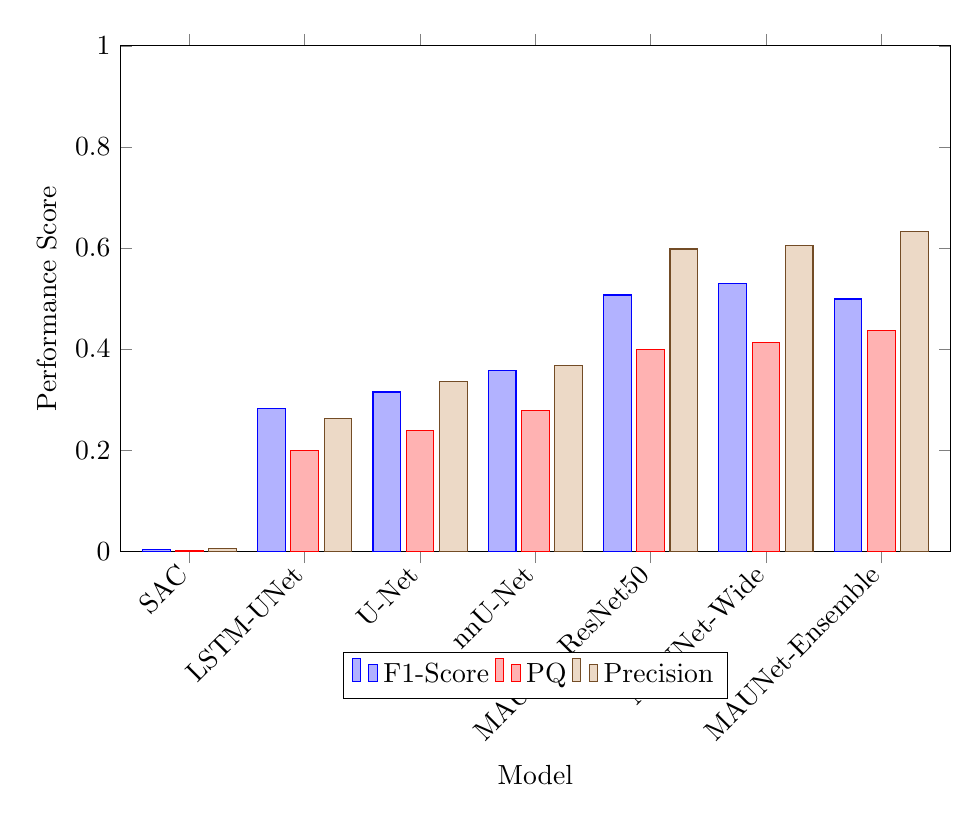
\begin{tikzpicture}
\begin{axis}[
    ybar,
    width=\textwidth,
    height=8cm,
    xlabel={Model},
    ylabel={Performance Score},
    symbolic x coords={SAC, LSTM-UNet, U-Net, nnU-Net, MAUNet-ResNet50, MAUNet-Wide, MAUNet-Ensemble},
    xtick=data,
    x tick label style={rotate=45, anchor=east},
    legend style={at={(0.5,-0.2)}, anchor=north, legend columns=3},
    ymin=0,
    ymax=1.0
]

% F1-Score bars
\addplot coordinates {
    (SAC, 0.003)
    (LSTM-UNet, 0.282)
    (U-Net, 0.315)
    (nnU-Net, 0.357)
    (MAUNet-ResNet50, 0.507)
    (MAUNet-Wide, 0.529)
    (MAUNet-Ensemble, 0.499)
};

% PQ bars
\addplot coordinates {
    (SAC, 0.002)
    (LSTM-UNet, 0.199)
    (U-Net, 0.239)
    (nnU-Net, 0.278)
    (MAUNet-ResNet50, 0.399)
    (MAUNet-Wide, 0.413)
    (MAUNet-Ensemble, 0.437)
};

% Precision bars
\addplot coordinates {
    (SAC, 0.005)
    (LSTM-UNet, 0.263)
    (U-Net, 0.335)
    (nnU-Net, 0.367)
    (MAUNet-ResNet50, 0.598)
    (MAUNet-Wide, 0.605)
    (MAUNet-Ensemble, 0.632)
};

\legend{F1-Score, PQ, Precision}
\end{axis}
\end{tikzpicture}
\caption{Model Performance Comparison Across Key Metrics}
\label{fig:performance_comparison}
\begin{quote}
\small
Comparative bar chart showing F1-Score, Panoptic Quality (PQ), and Precision across all evaluated models. MAUNet architectures demonstrate superior performance, with MAUNet-Ensemble achieving highest precision (0.632) and PQ (0.437), while MAUNet-Wide achieves best F1-Score (0.529). Traditional architectures (U-Net, nnU-Net) show moderate performance, while SAC exhibits poor performance across all metrics. The chart clearly illustrates the effectiveness of multi-scale attention mechanisms in cell instance segmentation tasks.
\end{quote}
\end{figure}
